\subsection{Момент импульса материальной точки и механической системы. Момент силы. Уравнение моментов. Закон сохранения момента импульса механической системы}

\begin{definition}
    Момент импульса материальной точки.
\end{definition}

\begin{wrapfigure}{l}{0.3\linewidth}
    \centering
    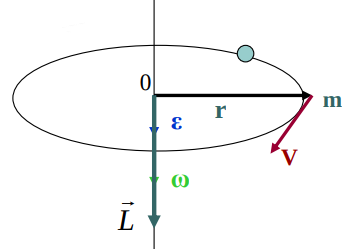
\includegraphics[width=\linewidth]{imgs/q8i1.png}
\end{wrapfigure}

Рассмотрим движение материальной точки массой $m$ по окружности радиуса $r$.

\begin{definition}
    Основное уравнение вращательного движения:

    $$
    I\cdot\varepsilon=M
    $$
\end{definition}

Учитывая, что:
$$
\begin{aligned}
    I = mr^2 \\
    \varepsilon = \frac{a_\tau}{r} \\
    a_\tau = \frac{dv}{dt}
\end{aligned}
$$

Получаем:

$$M=mr\frac{d\upsilon}{dt}$$

Внесём $mr$ под знак дифференциала, т.к. не зависит от $t$:

$$\frac{d(mr\upsilon)}{dt}=M$$

\begin{definition}
    Обозначим момент импульса материальной точки:
    $$L=mr\upsilon$$
\end{definition}

\begin{definition}
    Момент импульса — векторная величина, которая определяется как:
    $$\vec L=[\vec r\times\vec p]$$
\end{definition}

, где $\vec p=m\vec\upsilon$ - импульс материальной точки,
$\vec r$ - радиус-вектор

Для движения по окружности, $\vec r\perp\vec p$, поэтому

$$L=r\cdot p\ sin90^\circ=r\cdot p=mr\upsilon$$

Момент импульса системы точек 

$$L=\sum\limits_i [\vec{r_i}\times\vec{p_i}]$$

Момент импульса твёрдого тела.

$$\vec L=I\cdot\vec\omega$$

Момент импульса абсолютно твёрдого тела относительно оси вращения равен произведению его момента инерции относительно той же оси 
на угловую скорость.

\begin{definition}
    Момент силы относительно точки $[M_0, Н\cdot м]$ — векторная величина, 
    которая определяется векторным произведением радиус-вектора $\vec R$ и силы $\vec F$.
\end{definition}

$$\vec M_0=[\vec R,\vec F]=\vec R\times\vec F$$

Величина момента силы:

$$|\vec M_0|=|\vec R||\vec F|sin\alpha$$

\begin{definition}
    Закон сохранения момента импульса
    \begin{enumerate}
        \item В замкнутой механической системе.
        
        В замкнутых, изолированных механических системах вектор момента импульса сохраняется, т.е. не меняется с течением времени.
        $$\sum_i\vec L_i=const$$

        \item В частично замкнутой механической системе.
        $$\begin{cases}
            \sum\limits_i\frac{d\vec{L_{ix}}}{dt} = \vec{0} \\
            \sum\limits_i\frac{d\vec{L_{iy}}}{dt} = \vec{0} \\
            \sum\limits_i\frac{d\vec{L_{iz}}}{dt} = \vec{0} 
        \end{cases} \implies
        \begin{aligned}
            \sum\limits_i L_{ix} = const \\
            \sum\limits_i L_{iy} \neq const \\
            \sum\limits_i L_{iz} \neq const 
        \end{aligned}$$
    \end{enumerate}
\end{definition}

